\documentclass[hyperref={pdfpagemode=UseOutlines}]{beamer}
\usetheme{Madrid}

\usepackage[utf8]{inputenc} % unicode support
\usepackage{lmodern} % enable different font sizes
\usepackage{stmaryrd} % more symbols
\usepackage{amsmath,amsfonts,amssymb} % maths
\usepackage{mathtools} % maths operators
\usepackage{faktor} % quotient rings
\usepackage{graphicx} % graphics
\usepackage{float} % define floating objects like tables or figures
\usepackage{tikz} % draw images
\usepackage{booktabs} % table lines
\usepackage{url} % website links
\usepackage{csquotes} % quotes
\usepackage{multicol} % multicolumns for itemize
\usepackage[backend=biber,sorting=none,style=alphabetic]{biblatex} % references
\usepackage[linesnumbered, ruled]{algorithm2e} % algorithm package
\usepackage{aliascnt} % alias counter package

% macros
\newcommand{\mc}[1]{\multicolumn{1}{c}{#1}} % handy shortcut macro
\setbeamertemplate{itemize subitem}[triangle]

% maths operators
\DeclareMathOperator{\ord}{ord}
\DeclareMathOperator{\poly}{poly}
\DeclarePairedDelimiter{\abs}{\lvert}{\rvert}
\DeclarePairedDelimiter{\norm}{\lVert}{\rVert}
\DeclarePairedDelimiter{\paren}{(}{)}
\DeclarePairedDelimiter{\bkt}{[}{]}
\DeclarePairedDelimiter{\set}{\{}{\}}
\DeclarePairedDelimiter{\innerprod}{\langle}{\rangle}

% counters
\newcounter{savenumi}
\newcommand{\seti}{\setcounter{savenumi}{\value{enumi}}}
\newcommand{\conti}{\setcounter{enumi}{\value{savenumi}}}
\newaliascnt{mycounter}{algocf} % let "counter" be an alias for "algocf"
\newcommand\addtag{\refstepcounter{mycounter} \tag{\themycounter}}
\numberwithin{equation}{mycounter} % subordinate equations to mycounter
\numberwithin{table}{mycounter}

% algorithms
\SetKwInOut{Initialization}{Initialization}

% url
\def\UrlBreaks{\do/\do-}

% bibliography
\addbibresource{references.bib}

% title page before section
\AtBeginSection[]
{
    \begin{frame}
        \vfill
        \centering
        \begin{beamercolorbox}[sep=8pt,center,shadow=true,rounded=true]{title}
            \usebeamerfont{title} Section~\thesection:~\secname
        \end{beamercolorbox}
        \vfill
    \end{frame}
}

\AtBeginSubsection[]
{
    \begin{frame}
        \tableofcontents[sections=\thesection,currentsubsection]
    \end{frame}
}

\title{Beamer Template}
\author{Sim Jun Jie}

\begin{document}

\frame{\titlepage}

\begin{frame}[allowframebreaks]{Contents}
    \tableofcontents[hideallsubsections]
\end{frame}

\section{Slides Format}
\begin{frame}{Slides Format}{Beamer Template}
    \begin{itemize}
        \item Motivation
        \item Preliminaries
        \item Methods
        \item Results
    \end{itemize}
\end{frame}

\subsection{Motivation}
\begin{frame}{Motivation}{Slides Format}
    \begin{itemize}
        \item Discuss motivation
    \end{itemize}
\end{frame}

\subsection{Preliminaries}
\begin{frame}{Preliminaries}{Slides Format}
    \begin{itemize}
        \item Describe preliminaries needed
    \end{itemize}
\end{frame}

\subsection{Methods}
\begin{frame}{Methods}{Slides Format}
    \begin{itemize}
        \item Share method used
    \end{itemize}
\end{frame}

\subsection{Results}
\begin{frame}{Results}{Slides Format}
    \begin{itemize}
        \item Provide results
    \end{itemize}
\end{frame}

\section{Tables}
\begin{frame}{Tables}{Beamer Template}
    \begin{table}[H]
        \centering
        \caption{This is a table.}
        \begin{tabular}{lcccc}
            \toprule
             & col $1$ & col $2$ & col $3$ & col  $4$ \\
            \midrule
            row $1$ & $(1,1)$ & $(1,2)$ & $(1,3)$ & $(1,4)$ \\
            row $2$ & $(2,1)$ & $(2,2)$ & $(2,3)$ & $(2,4)$ \\
            row $3$ & $(3,1)$ & $(3,2)$ & $(3,3)$ & $(3,4)$ \\
            \bottomrule
        \end{tabular}
        \label{table1}
    \end{table}
\end{frame}

\section{Algorithms}
\begin{frame}{Algorithms}{Beamer Template}
    \begin{figure}
        \centering
        \begin{minipage}{0.8\linewidth}
            \begin{algorithm}[H]
                \caption{This is an algorithm.}
                \label{algo1}
                \KwIn {Some inputs}
                \KwOut {Some outputs}
                \Initialization {Some variables}

                \While {condition not met}
                {
                    Some code\;
                    Some more code\; \label{line1}
                }
                \For {$i = 0$ \KwTo $k$}
                {
                    \uIf {some condition holds}
                    {
                        Do some magic\;
                    }
                    \Else
                    {
                        \Return $m$\;
                    }
                }
            \end{algorithm}
        \end{minipage}
    \end{figure}
\end{frame}

\section{Citations}
\begin{frame}{Citations}{Beamer Template}
    \begin{itemize}
        \item Cite stuff like \cite{article} and \cite{misc}.
        \item Combine citations like\cite{book,incollection}.
    \end{itemize}
\end{frame}

\section{Images}
\begin{frame}{Images}{Beamer Template}
    \begin{figure}
        \begin{minipage}{\textwidth}
            \centering
            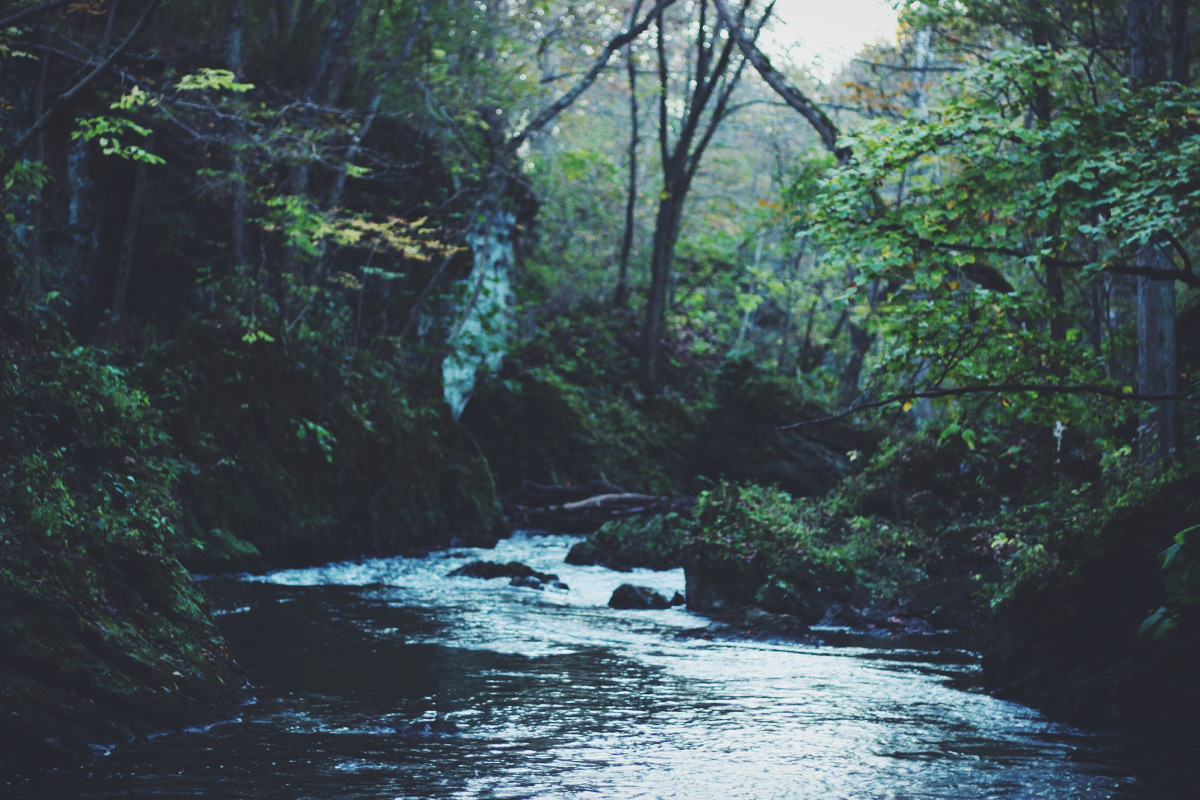
\includegraphics[width=0.8\textwidth,height=15em]{stream.jpg}
            \caption{Caption for image}
            \label{fig:sample_figure}
        \end{minipage}
    \end{figure}
\end{frame}

\section{References}
\begin{frame}[allowframebreaks]{References}
    \nocite{*}
    \printbibliography
\end{frame}

\begin{frame}
    \centering \Large
    \emph{Thank you}
\end{frame}

\end{document}